\chapter{Overview of \gls{athlet} and \gls{nut} software}\label{chapter:athlet-nut}

\section{\gls{athlet}}
\label{sec:athlet-overview}


The thermal-hydraulic system code \acrshort{athlet} (Analysis of THermal-hydraulics of LEaks and Transients) is developed by \acrshort{grs} for the analysis of the whole spectrum of operational conditions, incidental transients, design-basis accidents and beyond design-basis accidents without core damage anticipated for nuclear energy facilities \cite{grs:athlet-info}. The code provides specific models and methods for the simulation of many types of nuclear power plants comprising current light water reactors (PWR\footnote{Pressurized Water Reactor}, BWR\footnote{Boiling Water Reactor}, WWER\footnote{Water-Water Energetic Reactor}, HPCR\footnote{High Power Channel-type Reactor}), advanced Generation III+ and IV reactors as well as SMRs\footnote{Small Modular Reactor} \cite{grs:athlet-info}.\\


Physical processes inside of hydraulic circuits of light-water reactors can be naturally described by a two-phase thermo-fluiddynamic model based on conservation equations of mass, momentum and energy for liquid and vapor.\\

1. Liquid mass
\begin{equation} \label{eq:athlet-1}
\frac{\partial ((1-\alpha)\rho_{l})}{\partial t} + \nabla ((1-\alpha) \rho_{l} \vec{w_{l}}) = - \psi
\end{equation}


2. Vapor mass
\begin{equation} \label{eq:athlet-2}
\frac{\partial (\alpha \rho_{v})}{\partial t} + \nabla (\alpha \rho_{v} \vec{w_{v}}) = \psi
\end{equation}


3. Liquid momentum
\begin{equation} \label{eq:athlet-3}
\frac{\partial ((1-\alpha) \rho_{l} \vec{w_{l}})}{\partial t} + \nabla ((1-\alpha) \rho_{l} \vec{w_{l}} \vec{w_{l}}) + \nabla ((1 - \alpha)p) = \vec{F_{l}}
\end{equation}


4. Vapor momentum
\begin{equation} \label{eq:athlet-4}
\frac{\partial (\alpha \rho_{v} \vec{w_{v}})}{\partial t} + \nabla (\alpha \rho_{v} \vec{w_{v}} \vec{w_{v}}) + \nabla (\alpha p) = \vec{F_{v}}
\end{equation}


5. Liquid energy
\begin{equation} \label{eq:athlet-5}
\frac{\partial \Big[ (1-\alpha)\rho_{l}(h_{l} + \frac{1}{2} \vec{w_{l}} \vec{w_{l}} - \frac{p}{\rho_{l}}) \Big]}{\partial t} + \nabla \Big[ (1-\alpha)\rho_{l}\vec{w_{l}}(h_{l} + \frac{1}{2} \vec{w_{l}} \vec{w_{l}}) \Big] = - p \frac{\partial (1 - \alpha)}{\partial t} + E_{l}
\end{equation}


6. Vapor energy
\begin{equation} \label{eq:athlet-6}
\frac{\partial \Big[ \alpha \rho_{v}(h_{v} + \frac{1}{2} \vec{w_{v}} \vec{w_{v}} - \frac{p}{\rho_{v}}) \Big]}{\partial t} + \nabla \Big[ \alpha\rho_{v}\vec{w_{v}}(h_{v} + \frac{1}{2} \vec{w_{v}} \vec{w_{v}}) \Big] = - p \frac{\partial \alpha}{\partial t} + E_{v}
\end{equation}

7. Volume vapor fraction
\begin{equation} \label{eq:athlet-7}
	\alpha = \frac{V_{v}}{V}
\end{equation}


where $p$ - pressure of mixture, $\psi$ - mass source term, $\vec{F}$ - external composite force acted on a control volume, $E$ - external composite energy source term within a control volume, subscripts $l$ and $v$ denote liquid and vapor phases, respectively. \\


% Finite volume and 1D discritiazation 
Spacial integration of the conservation equations, the ssystem \ref{eq:athlet-1} - \ref{eq:athlet-7}, is performed on the basis of finite-volume method with using one dimensional formulation, figure \ref{fig:introduction-1d-fvm}.


\figpointer{\ref{fig:introduction-1d-fvm}}
\begin{figure}[htpb]
  \centering
  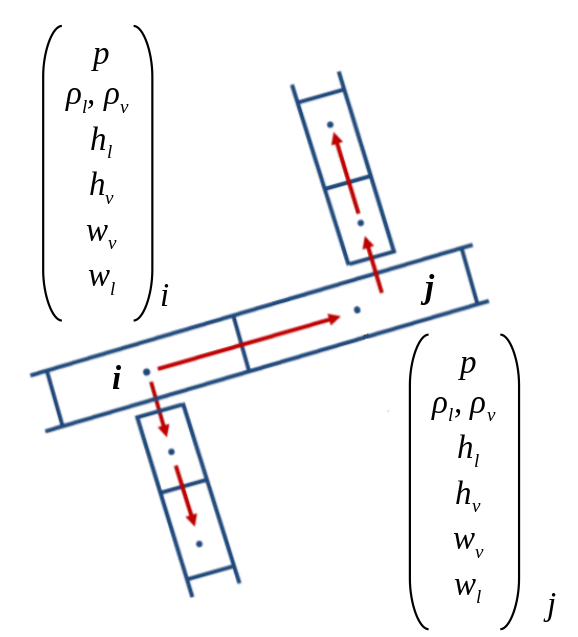
\includegraphics[width=0.55\textwidth]{figures/introduction-1d-fvm.png}
\caption{One dimensional finite volume formulation of thermo-hydraulic modeling in \acrshort{athlet}, \cite{tims-presentation}}
\label{fig:introduction-1d-fvm}
\end{figure}


Finally, the system is transformed to a non-autonomous system of ordinary differential equations and expressed as an initial value problem, equation \ref{eq:athlet-8}, after spatial finite-volume integration and many mathematical transformations \cite{lt:ATHLMaM}. 


\begin{equation} \label{eq:athlet-8}
	\frac{dy}{dt} = f(t,y), \;  t_{0} \leq t \leq t_{F} \; y(t_{0}) = y_{0}
\end{equation}

where $y \in \mathbb{R}^{N}$ is a composite vector of variables, $f$ is a non-linear function such that $f : \mathbb{R} \times \mathbb{R}^{N} \supset \Omega  \rightarrow \mathbb{R}^{N}$  .\\


% Rosenbrock-Wanner
Analysis of system \ref{eq:athlet-8} shows the problem is rather and thus must to be solved with an implicit solver. Rosenbrock methods are a class of linear implicit methods which is capable of solving such stiff systems of \acrshort{ode}s efficiently. The methods replace non-linear systems with a sequence of linear ones, however, some stability and accuracy properties are usually lost \cite{blom2013rosenbrock}. An additional drawback of the methods is evaluation of the exact Jacobian at every time step which affects computational cost.\\


To decrease the cost and preserve sufficient accuracy of numerical integration, \acrshort{athlet}, instead, uses a W-method of the third order. W-methods belong to the family of Rosenbrock methods, however, calculate the Jacobian matrix occasionally. The \acrshort{athlet} developers spent much of their time and efforts to develop heuristics to identify instances of time when evaluation of the Jacobian must be performed. In other words, the algorithm can re-use the same Jacobian matrix approximation between steps with some partial matrix updates. However, when a hydraulic circuit state drastically changes due to transitivity, the evaluation of the full Jacobian is demanded.\\


\figpointer{\ref{fig:introduction-w-method-scheme}}
\begin{figure}[htpb]
  \centering
  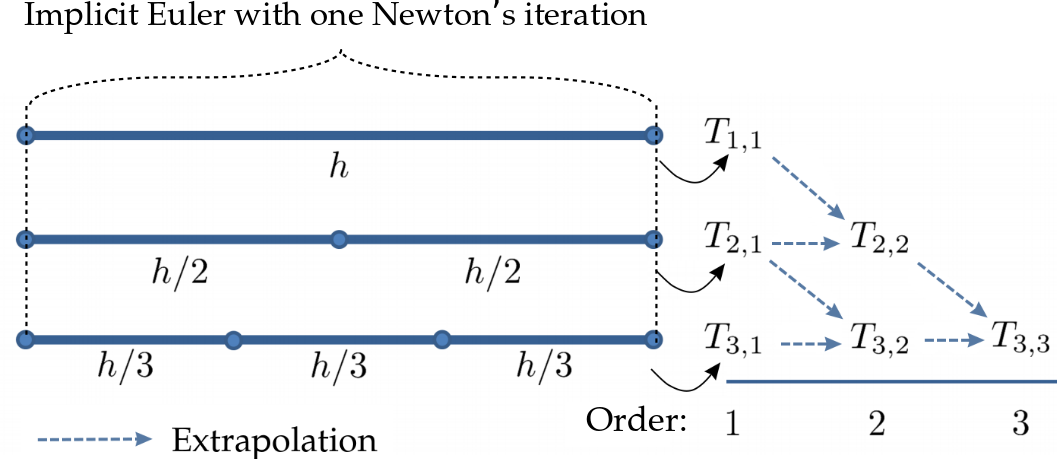
\includegraphics[width=0.8\textwidth]{figures/introduction-rosenbrock-scheme.png}
\caption{A general view on the 6-stage W-method implemented in \acrshort{athlet}}
\label{fig:introduction-w-method-scheme}
\end{figure}


In the general case, a step of the W-method method, implemented in \acrshort{athlet}, can be viewed as a sequence of six stages in the following way. Each stage uses implicit Euler method and exactly one Newton's iteration to evaluate the value of vector $y$ at the next integration step $h$ with different accuracy. Then, the obtained values are extrapolated, in order explained in figure \ref{fig:introduction-w-method-scheme}, to achieve desired order of integration. By and large, the algorithm can be expressed in a compact form of equation \ref{eq:athlet-9}.

\begin{equation} \label{eq:athlet-9}
	((h \gamma)^{-1}I - J) \Delta z^{l}_{i} = - h^{-1} z^{l}_{i} + f(t_0 + \tau_{i} h, y_{0} + z^{l}_{i})
\end{equation}

where $\Delta z^{l}_{i} = z^{l+1}_{i} - z^{l}_{i}$, $z^{l}_{i} = y^{l}_{i} - y^{l}_{i - 1}$, $J \approx \frac{\partial f}{\partial y}$ - approximation of Jacobian matrix, $l = 1,2$ - Newton's iteration index, $i = 1, 2, 3$ - integration step index.\\


\section{\acrshort{nut}}

Numerical Toolkit, or just \acrshort{nut}, can be viewed as a container of various dense and sparse linear algebra subroutines which can run in parallel on distributed-memory machines. \acrshort{nut} design follows the paradigm of \textit{Adapter/Wrapper} pattern which provides a uniform common interface for its services to various \acrshort{grs} simulation tools (outlined in table \ref{table:introduction-grs-software}) and thus helps to achieve re-usability, flexibility and extensibility properties of the code.\\


Currently, \acrshort{nut} is based heavily on Portable, Extensible Toolkit for Scientific Computation, known as \acrshort{petsc} library. It is one of the most widely used parallel numerical software  library \cite{wiki:petsc-general-info}. It includes a large suite of parallel linear and nonlinear equation solvers as well as its software-infrastructure to handle computations on distributed-memory machines by means of Message Passing Interface (\acrshort{mpi}) and specific data structures. Fortunately, though a careful selection of the design pattern, \acrshort{nut} can be easily extended to provide an extra service or an external library access which has not been implemented in \acrshort{petsc} yet.\\ 


\section{\acrshort{athlet}-\acrshort{nut} coupling}
\label{sec:athlet-nut-coupling}

\figpointer{\ref{fig:introduction-nut-process-groups}}
\begin{figure}[htpb]
  \centering
  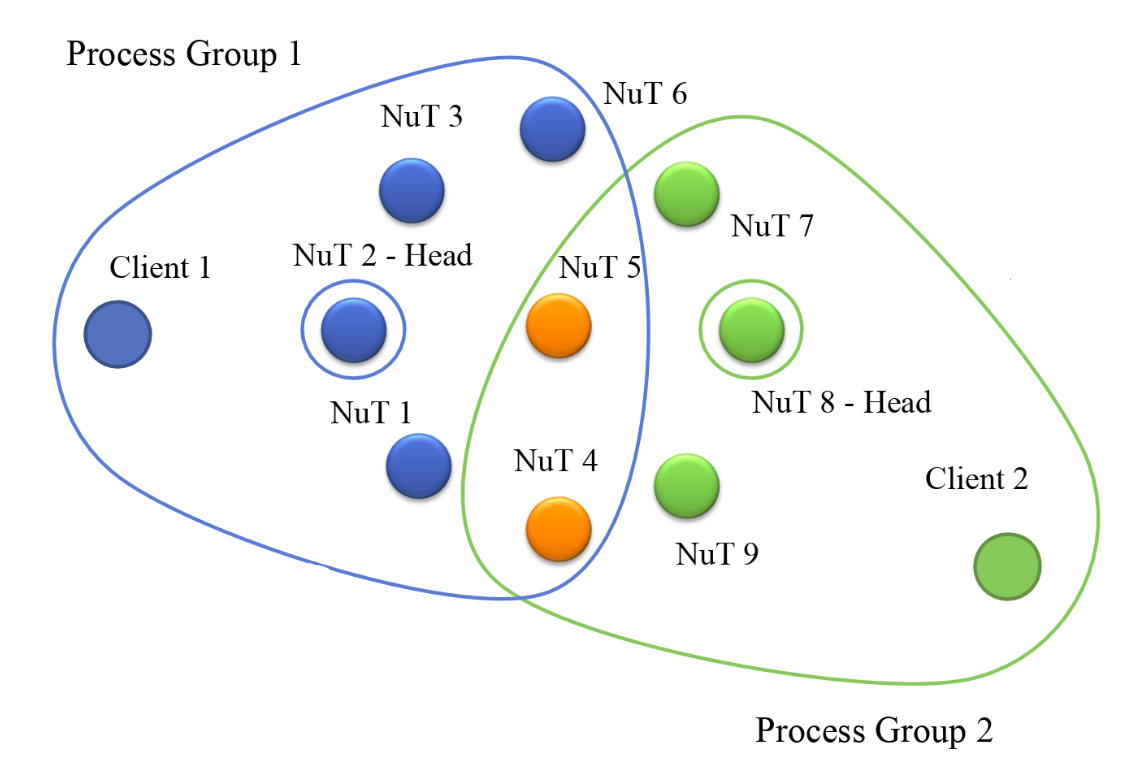
\includegraphics[width=0.8\textwidth]{figures/introduction-nut-process-groups.png}
\caption{An example of \acrshort{nut} process groups}
\label{fig:introduction-nut-process-groups}
\end{figure}

Coupling of \acrshort{nut} with \acrshort{grs} tools is based on the client-server architecture where \acrshort{nut} acts as a server and the tools can be viewed as clients. Communication between two parts is done via \acrshort{mpi}.\\


To provide a clear and concise external interface, \acrshort{nut} contains a client module called "\acrshort{nut} Plug-in". It can be  considered as a socket, from the client side, using the analogy of Transmission Control Protocol (TCP). The plug-in hides all \acrshort{mpi} calls to the sever which considerably improves readability of the code.\\


% communicators
In the general case, \acrshort{nut} allows multiple clients to work concurrently with the server. To handle the traffic, the library splits the default \acrshort{mpi} communicator at start-up time of the application into appropriate process groups, as it is shown in figure \ref{fig:introduction-nut-process-groups}.\\



The design of \acrshort{nut} allows sharing of some \acrshort{nut}-\acrshort{mpi} processes among different process groups due to performance reasons i.e. finite number of processing units on hardware. To resolve possible deadlocks, each process group has its own representative, called the head. Each client has two views on its respective group which is achieved by means of distinct \acrshort{mpi} communicators. The first communicator is responsible for client-head communication whereas the second one allows the client to talk to any \acrshort{nut} process within the group.\\



A general view of client-server communication looks like a 3-way handshake in the following way: a client sends a request to the head which is a signal to reserve all compute-units of the group for an upcoming task. Having possessed the resources and prepared them for a specific service, the head notifies the client about resource acquisition and the entire process group waits for data. Afterwards, the client sends data either to a specific \acrshort{nut}-process or to the entire group using the second communicator and waits for a result of the service. In the current implementation of \acrshort{nut}, the communication between client and server is synchronous i.e. the client gets blocked while waiting for a result from the server. \\


As an example, figure \ref{fig:introduction-athlet-nut-coupling} represents a general view of \acrshort{athlet}-\acrshort{nut} coupling where \acrshort{athlet} is responsible for marching of the numerical integration solver whereas \acrshort{nut} computes solutions of systems \ref{eq:athlet-9}.\\


\figpointer{\ref{fig:introduction-athlet-nut-coupling}}
\begin{figure}
  \centering
  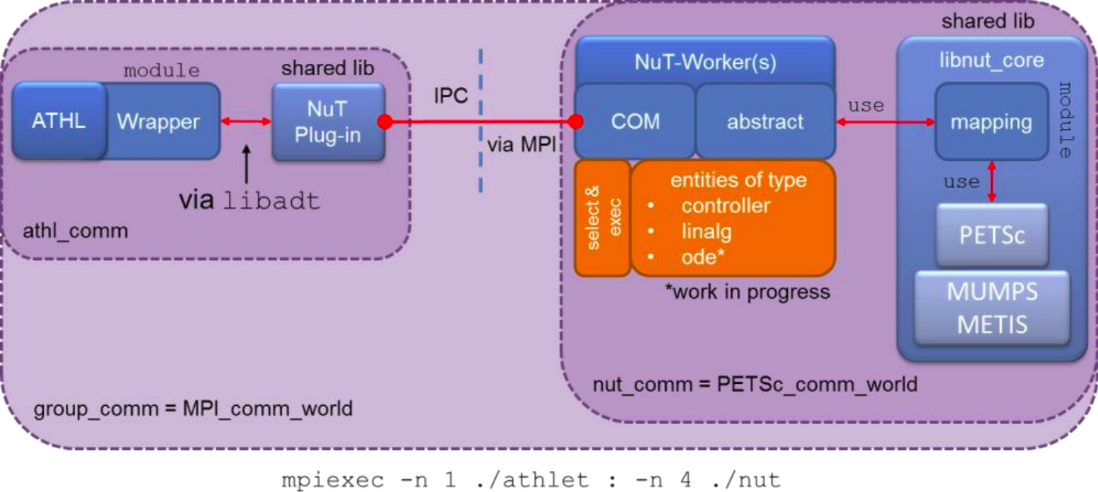
\includegraphics[width=0.75\textwidth]{figures/introduction-athlet-nut-coupling.png}
    \caption{\acrshort{athlet}-\acrshort{nut} software coupling}
\label{fig:introduction-athlet-nut-coupling}
\end{figure}


Partial and full Jacobian matrix updates derived from finite differences are computed on the client side since only the client has the access to function $f(y)$, equation \ref{eq:athlet-8}. Due to decoupling of the underlying system of \acrshort{pde}s and specifics of finite volume discretization, Jacobian matrix is rather sparse and, therefore, \acrshort{athlet} uses a Jacobian matrix compression algorithm, described in section \ref{sec:jacobian-matrix-compression}, to reduce the amount of Jacobian column evaluations. Having computed a matrix column, \acrshort{athlet} immediately broadcasts it to its entire \acrshort{nut} process group by means of 3-way handshake mechanism as described above. It is worth mentioning that this approach allows to circumvent potential memory limits on the client side and thus store the entire sparse Jacobian matrix in a distributed fashion on the server. In other words, \acrshort{athlet} never holds the entire Jacobian matrix in its memory; conversely, the matrix is distributed across multiple \acrshort{nut} processes according to block-row distribution induced by \acrshort{petsc}. In turn, \acrshort{nut} is waiting for the entire Jacobian matrix information from \acrshort{athlet} and starts solving systems \ref{eq:athlet-9} right after the corresponding request from the client.\\


